\chapter{Experimental Evaluation}
\label{cap:evaluation}

This chapter presents the results of a set of experimental tests performed to
evaluate the overheads introduced by the exploitation of the proposed process
migration mechanism.

The overheads may be categorized in two types: performance loss due to the
execution of multiple \emph{ORTE daemons} on the same node and the time
required to actually perform the process migration.

For each performance test, in this Chapter we provide the description of the software used, the hardware setup, the methodology applied to perform the measures and finally the results obtained.

\section{Introduction}
As we have discussed in Subsection \ref{subsec:multipleorted}, the execution of
multiple \emph{ORTE daemons} on the same node enables the migration of a subset
of processes instead of migrating the entire population of processes running
on the same node. This
ensures higher flexibility both for the system resource management and the
wide range of use cases that can benefit from a task migration mechanism. The
advantages have been previously described in
Subsection \ref{subsec:multipleorted}.
Unfortunately, there are also drawbacks, in terms of overheads impact on the
application execution. Splitting the control of the application processes
lifecycle under different \emph{ORTE daemons} in facts, implies that some processes cannot rely
anymore on shared memory to communicate with each other, even if they are
running on the same node. In such cases, we need to use TCP/IP connections for
inter-process communication, which have been shown to be less performing than
shared memory \cite{graham2005open}.

In Section \ref{sec:migoverhead} instead, the migration overhead is presented.
It represents the time lost to complete all the migration procedure described
in Chapter \ref{cap:design}. Therefore, opposite to the multiple \emph{ORTE
daemons} overhead, the migration overhead is not a persistent overhead. It
impacts on the application execution time only if the migration is triggered.

Finally, in Section \ref{sec:distribval} we show the validation of the DistRib
policy of the BarbequeRTRM discussed in Section \ref{sec:distribpolicy}.

\subsection{The NAS Parallel Benchmark Suite}
The \textbf{NAS Parallel Benchmark Suite (NPB)} \cite{bailey1991parallel} is
a benchmark suite developed by the \emph{NASA Advanced Supercomputing
Division} since 90s. This set of applications is designed to evaluate the
performance of supercomputers that exploits the parallel computation. The
benchmarks are implemented with several technologies, such as \emph{MPI},
\emph{OpenMP}, \emph{Java}, \emph{HPF}\footnote{High Performance Fortran is
an extension of Fortran 90 for parallel applications.}, Globus. However,
only the \emph{MPI} and \emph{OpenMP} implementations are continuously
developed and updated. They do not depend on a particular implementation 
of \emph{MPI} and \emph{OpenMP}.

The NPB suite is widespread acknowledged in research, therefore
we used it for testing both the multiple \emph{ORTE daemons} overhead
and the migration overhead. We selected the original eight benchmarks specified in NPB version
1, composed of five kernels and three pseudo applications. NPB version 2 and 3
introduced also other special benchmarks:
\begin{itemize}
\item NPB-MZ: the multi-zone version of the original pseudo-applications;
\item The unstructured computation benchmarks;
\item The parallel I/O benchmarks for specific techniques;
\item GridNPB to test the performance of computational grids.
\end{itemize}
Since these specific benchmarks are not significant for our migration
mechanism, we decided to use only a subset of the original benchmarks.

The original five kernels are focused on testing the performance on
particular metrics, instead the pseudo-applications are common abstractions
of real problems solvable with MPI frameworks:
\begin{itemize}
\item \textbf{Kernels}
\begin{itemize}
\item \emph{Integer Sort} (\texttt{IS}): parallel sort of uniform distributed integer 
      keys. It provides a balanced benchmark on integer computation,     random memory and network communication speeds.
\item \emph{Embarrassingly Parallel} (\texttt{EP}): generation of pairs of Gaussian
	  deviates. It provides an estimation of floating-point performance 
	  upper-limit. The inter-process communication is minimal and
	  non-significant.
\item \emph{Conjugate Gradient} (\texttt{CG}): application of the Inverse Power Method
      to find the largest eigenvalue of a sparse randomized matrix. It tests
      the performance of irregular memory accesses and irregular long-distance
      communications.
\item \emph{Multi-Grid} (\texttt{MG}): an ad-hoc multigrid algorithm to solve the
	   Poisson Problem \(\nabla^2u=v\). It is a good representation of the
	   performance of long- and short-distance communication and memory
	   intensive operations.
\item \emph{Fourier Transform} (\texttt{FT}): solving a Partial Differential Equation
      using forward and inverse Fast Fourier Transformations. It is a rigorous 
      test of long-distance all-to-all communication performance.
\end{itemize}
\item \textbf{Pseudo-Applications}
\begin{itemize}
\item \emph{Block Tri-diagonal solver} (\texttt{BT})
\item \emph{Scalar Penta-diagonal solver} (\texttt{SP})
\item \emph{Lower-Upper Gauss-Seidel solver} (\texttt{LU})
\end{itemize}

\end{itemize}

Every kernels have integrated verification tests. These tests may be 
\emph{partial verification} - if they are conducted on partial results - or 
\emph{full verification} - if they are conducted after the combination of
all partial results. As a consequence, we can also verify if the migration
procedure has corrupted the application execution.

The benchmarks use a dedicated Pseudorandom Number Generator in order to
generate uniform distributed pseudorandom numbers. This algorithm ensures 
sufficient randomicity, independently on the system used for executing the
suite, provided some system constraints are met. However, most of the systems
in use today meet these requirements.

%\def\arraystretch{1.3}%
\begin{table}[t]
\centering
\begin{tabular}{c| R{1.3cm} R{1.3cm} R{1.3cm} R{1.3cm} R{1.3cm} R{1.3cm} R{1.2cm}} \cline{2-8}
\multicolumn{1}{c}{} & \multicolumn{7}{c}{\textbf{Class }} \\ \cline{1-8}
\multicolumn{1}{c|}{\textbf{Bench.}} & \textbf{S} & \textbf{W} & \textbf{A}
 & \textbf{B} & \textbf{C} & \textbf{D} & \textbf{E}\\ \hline
\texttt{IS} & 512 KB  & 8 MB  & 64 MB     & 256 MB    & 1 GB    & 16.4 GB & N.A. \\
\texttt{EP} & 128 MB  & 256 MB  & 2 GB     & 8 GB    & 32 GB & 512 GB & 8 TB \\
\texttt{CG} & 76.6 KB & 437 KB  & 1.2 MB     & 7.4 MB    & 172 MB & 240 MB & 1.7 GB \\
\texttt{MG} & 256 KB & 16 MB & 128 MB    & 128 MB    & 1 GB    & 8.1 GB & 64 GB \\
\texttt{FT} & 2 MB  & 4 MB  & 64 MB     & 256 MB    & 1 GB & 16 GB & 128 GB \\

\texttt{BT} & 13.5 KB & 108 KB
& 2 MB      & 8 MB      & 32 MB     & 518 MB & 8 GB \\
\texttt{LU} & 13.5 KB & 280 KB
& 2 MB      & 8 MB      & 32 MB     & 518 MB & 8 GB \\
\texttt{SP} & 13.5 KB & 364 KB
& 2 MB      & 8 MB      & 32 MB     & 518 MB & 8 GB \\ \hline
\end{tabular}
\caption[NPB problem data sizes]{Problem data sizes for each class and benchmark in NPB suite
\cite{NPBDataSize}.}
\label{tab:cap6-npb-classes}
\end{table}

Furthermore, each problem has multiple \textbf{classes} to be selected, where a class represents the input data size, summarized in Table
\ref{tab:cap6-npb-classes}.

% \subsection{Terminology}
% In order to clearly describe the executed performance tests,
% the following terms are used:
% \begin{itemize}
% \item \textbf{Wall-time}: the total application execution time, calculated
% starting from immediately after the variables initialization to immediately before the functions that performs output.
% \item \textbf{Granularity}: the average number of ORTE Daemons spawned on each
%                             node.
% \end{itemize}


\section{\texttt{mig}: \emph{ORTE daemons} granularity overhead}

\subsubsection{Hardware setup}
We used a computing node equipped with two Intel Xeon E5-2640 octa-core
hyper-threaded CPUs, with 128GB of RAM per CPU. The system is based on a NUMA
architecture.

As common in HPC environments, we disabled Hyper-Threading, remaining with
16 cores at our disposal. The running operating system was CentOS 6.7 with
updated Linux kernel version 3.18.

\subsubsection{Methodology}
We selected \texttt{IS}, \texttt{MG} kernels and \texttt{BT}, \texttt{SP},
\texttt{LU} pseudo-applications. We discarded the other kernels since their
execution would not be affected significantly by a run-time migration of
some processes:
\begin{itemize}
\item \texttt{EP} is not a good candidate for testing communication, since it
      does not almost send anything. 
\item \texttt{CG} tests long distance communication and our overhead is 
      present only in short distance (even same machine).
\item \texttt{FT} as for \texttt{CG} it tests only long distance and not short.
\end{itemize}


The kernels were executed specifying input classes \texttt{B}, \texttt{C},
\texttt{D}. For the pseudo-applications, instead, we did not
consider class
\texttt{D} since the completion of the execution would require too much time
using the systems at our disposal.
Finally, we excluded classes \texttt{S}, \texttt{W}, \texttt{A} because the problem size would have
been too small, leading to very short executions. Vice versa, \texttt{E} class
would be too expensive in terms of memory and execution time.

We executed the pairs \texttt{(benchmark, class)} spawning 16 processes for each
benchmark execution. We selected the number of \emph{ORTE daemons} controlling the
MPI processes according to different granularities: 1, 2, 4, 8, 16.
Each \emph{ORTE daemon} instance had therefore to manage 16, 8, 4, 2 or 1 MPI
processes respectively. In particular, the case of single \emph{ORTE daemon} instance
is a standard execution of unmodified Open MPI and we took it as a reference
result in the overhead evaluation.

We measured the execution time of each tuple \texttt{(benchmark, class,}\\
\texttt{granularity)}, starting after the \texttt{MPI\_Init} call and
stopping before the\\
\texttt{MPI\_Finalize} call. The time needed to
spawn the \emph{ORTE daemons} and the processes are therefore not considered. We
repeated the test 20 times to obtain a significant statistics. It turned out
that we experienced an average standard deviation below 1\% of the total
execution time.


\subsubsection{Results}
The overall results are shown in Figure \ref{fig:cap6-ortedstatic}. The global
trend is that the overhead increases sub-linearly with respect to the number
of \emph{ORTE daemon} instances, while it decreases as the problem size increases.
The sub-linear increase of the overhead can be explained by the fact that,
once there are at least two \emph{ORTE daemon} instances, the TCP/IP communication
between MPI processes on different instances becomes the bottleneck for
communication latencies.
Adding more \emph{ORTE daemon} instances to the existing ones does not tend to
further degrade performance.

Conversely, the decrease of the overhead in case of
increasing problem size is due to the fact that increasing
problem size means that more time is spent on computing data; therefore
the time spent in communication -- which is where the overhead applies
-- decreases in percentage.

Looking at the data summarized in Table \ref{tab:cap6-staticbench}, we can state that the \emph{ORTE daemons} granularity poorly
affects the application execution time. Considering all the test cases, we can
observe indeed that the percentage of time loss remains in the $0-5.x\%$ range.



\begin{figure*}[t]
\centering

\subfloat{%
   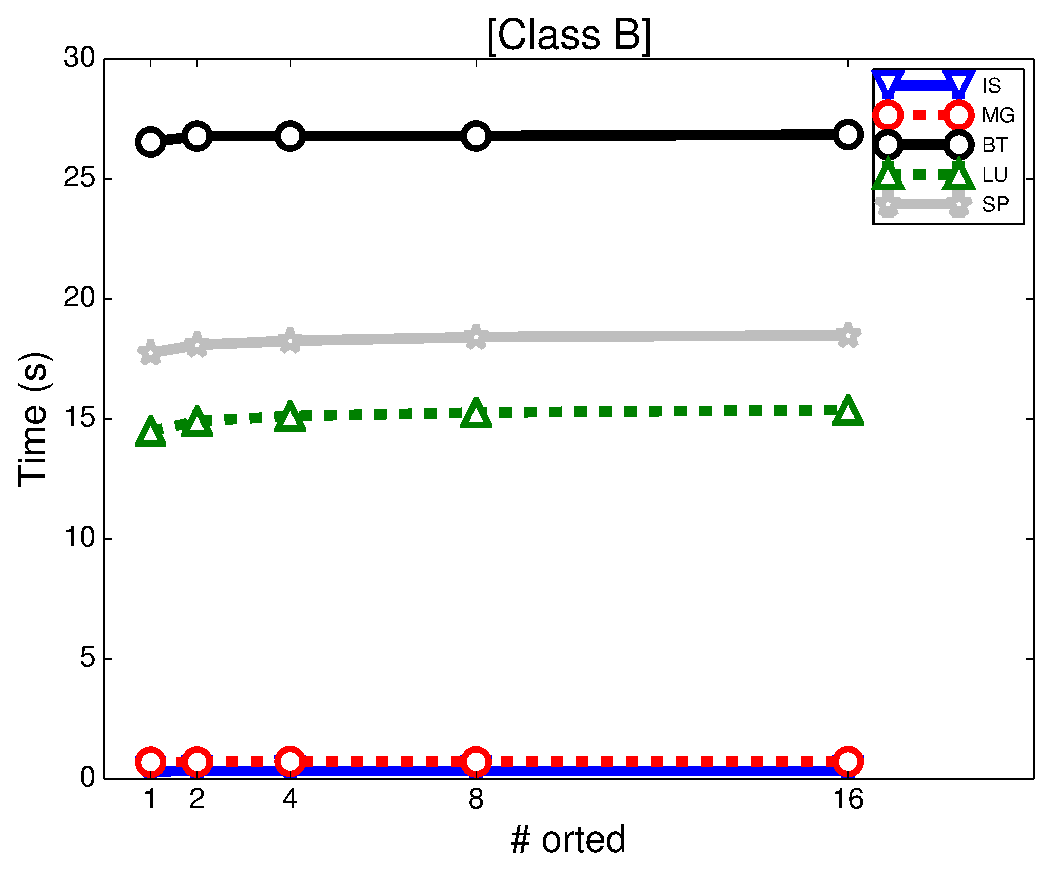
\includegraphics[scale=0.45]{img/orted_no_B_time.eps}
}
\hspace{3pt}
\subfloat{%
   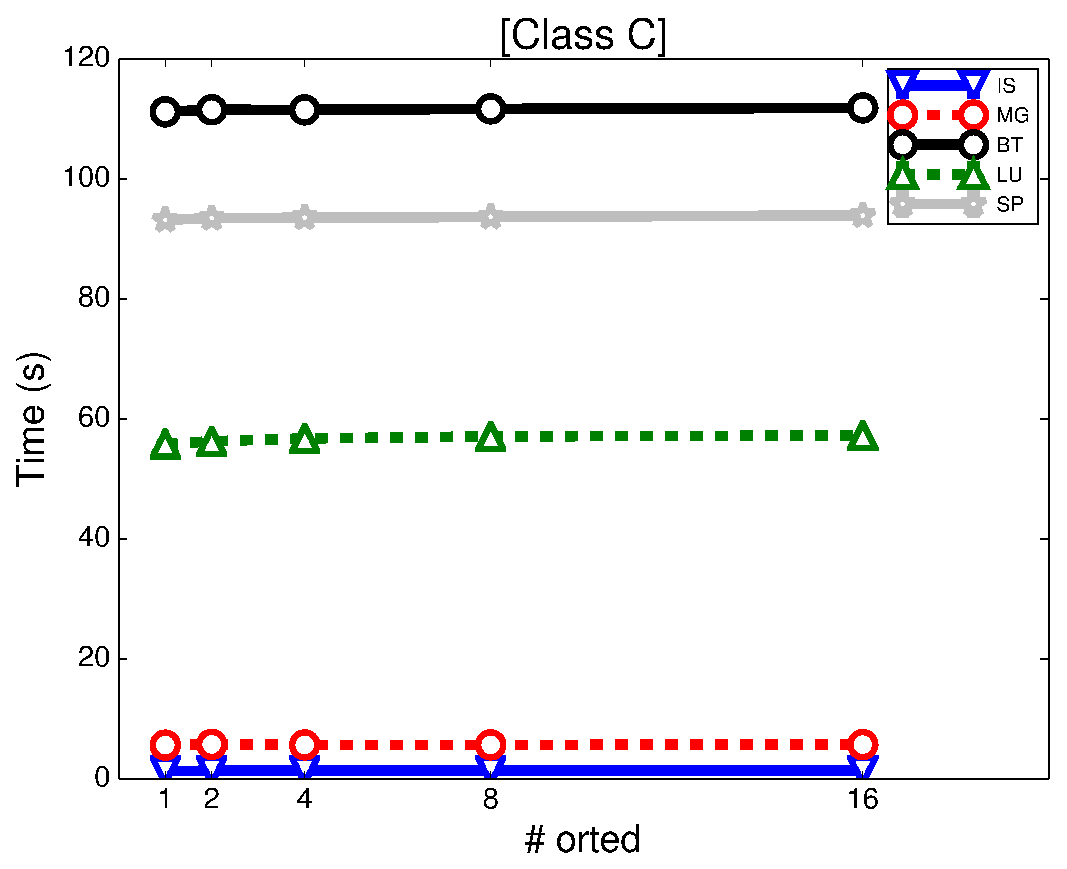
\includegraphics[scale=0.45]{img/orted_no_C_time.eps}
}
\hspace{3pt}
\subfloat{%
   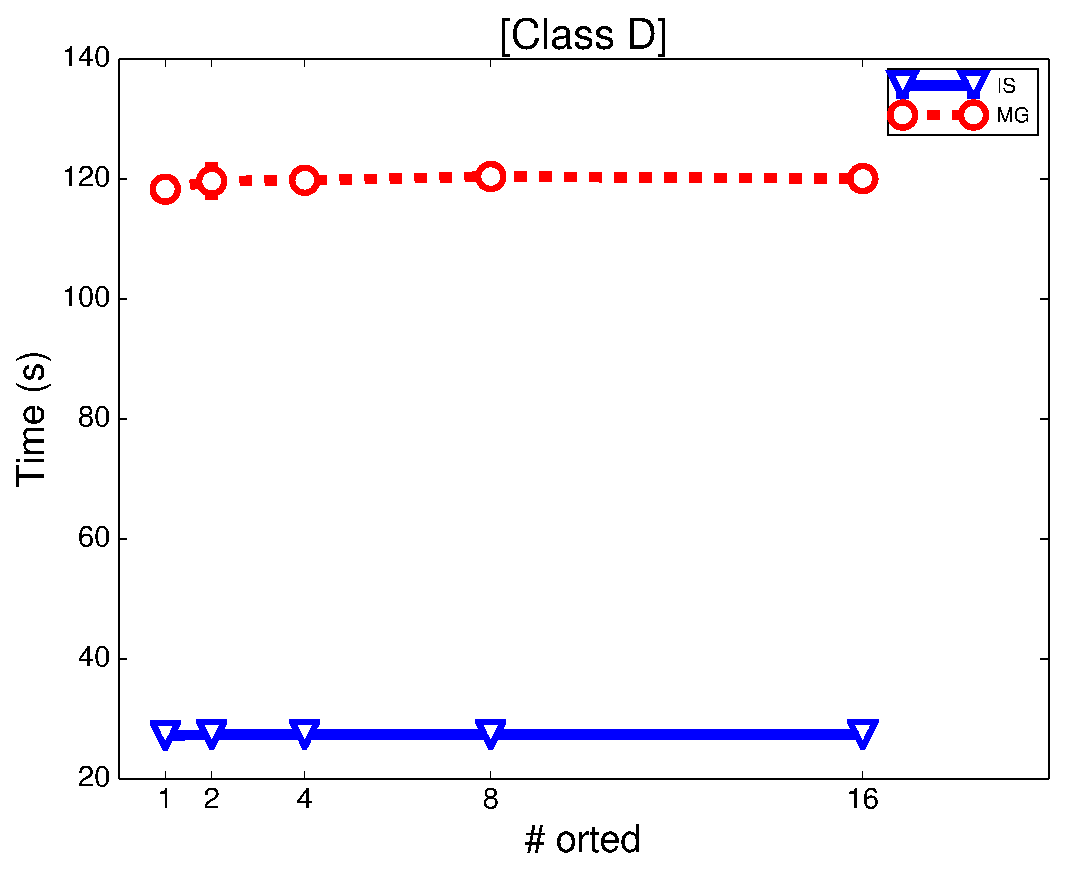
\includegraphics[scale=0.45]{img/orted_no_D_time.eps}
}
\caption[Multiple ORTE daemons benchmark]{Execution time of each benchmark when running 16 processes
using a number of \emph{ORTE daemons} that ranges from 1 to 16.}
  \label{fig:cap6-ortedstatic}%
\end{figure*}

\begin{table}[t]
\footnotesize
\centering
\begin{tabular}{c|c|c|C{2cm}} \hline
   \textbf{Benchmark} & \textbf{Class} &
   \begin{tabular}[x]{@{}c@{}}\textbf{\# orted}\end{tabular} &
         \begin{tabular}[x]{@{}c@{}}\textbf{Overhead} \textbf{\%}\end{tabular} \\ \hline

    \multirow{12}{*}{\texttt{IS}} & \multirow{4}{*}{B} & 2  & 4.68 \\
     &   & 4  & 5.18 \\
     &   & 8  & 4.85 \\
     &   & 16 & 4.85 \\ \cline{2-4}

     & \multirow{4}{*}{C} & 2  & 2.21 \\
     &   & 4  & 2.68 \\
     &   & 8  & 2.64 \\
     &   & 16 & 2.64 \\ \cline{2-4}

     & \multirow{4}{*}{D} & 2  & 0.87 \\
     &   & 4  & 0.96 \\
     &   & 8  & 0.79 \\
     &   & 16 & 0.64 \\ \hline

    \multirow{12}{*}{\texttt{MG}} & \multirow{4}{*}{B} & 2  & 1.28 \\
     &   & 4  & 4.36 \\
     &   & 8  & 1.73 \\
     &   & 16 & 3.24 \\ \cline{2-4}

     & \multirow{4}{*}{C} & 2  & 2.25 \\
     &   & 4  & 0.62 \\
     &   & 8  & 0.88 \\
     &   & 16 & 1.57 \\ \cline{2-4}

     & \multirow{4}{*}{D} & 2  & 1.13 \\
     &   & 4  & 1.25 \\
     &   & 8  & 1.79 \\
     &   & 16 & 1.50 \\ \hline

    \multirow{8}{*}{\texttt{BT}} & \multirow{4}{*}{B} & 2  & 0.92 \\
     &   & 4  & 0.93 \\
     &   & 8  & 0.93 \\
     &   & 16 & 1.17 \\ \cline{2-4}

     & \multirow{4}{*}{C} & 2  & 0.31 \\
     &   & 4  & 0.29 \\
     &   & 8  & 0.45 \\
     &   & 16 & 0.60 \\ \hline

    \multirow{8}{*}{\texttt{SP}} & \multirow{4}{*}{B} & 2  & 1.90 \\
     &   & 4  & 2.83 \\
     &   & 8  & 3.72 \\
     &   & 16 & 4.12 \\ \cline{2-4}

     & \multirow{4}{*}{C} & 2  & 0.31 \\
     &   & 4  & 0.40 \\
     &   & 8  & 0.52 \\
     &   & 16 & 0.79 \\ \hline

    \multirow{8}{*}{\texttt{LU}} & \multirow{4}{*}{B} & 2  & 2.92 \\
     &   & 4  & 4.37 \\
     &   & 8  & 5.42 \\
     &   & 16 & 6.10 \\ \cline{2-4}

     & \multirow{4}{*}{C} & 2  & 0.73 \\
     &   & 4  & 1.63 \\
     &   & 8  & 2.19 \\
     &   & 16 & 2.48 \\ \hline


\end{tabular}
\caption[Multiple ORTE daemons static overhead]{Static overhead of \texttt{IS}, \texttt{MG}, \texttt{BT}, \texttt{SP}, and \texttt{LU} with
increasing migration granularity, i.e. increasing number of \emph{ORTE daemons},
compared with single \emph{ORTE daemon} case.}
\label{tab:cap6-staticbench}
\end{table}

\clearpage


%% Migration composition
\begin{figure*}[t]
\centering
%\hspace{-53pt}
\subfloat{%
   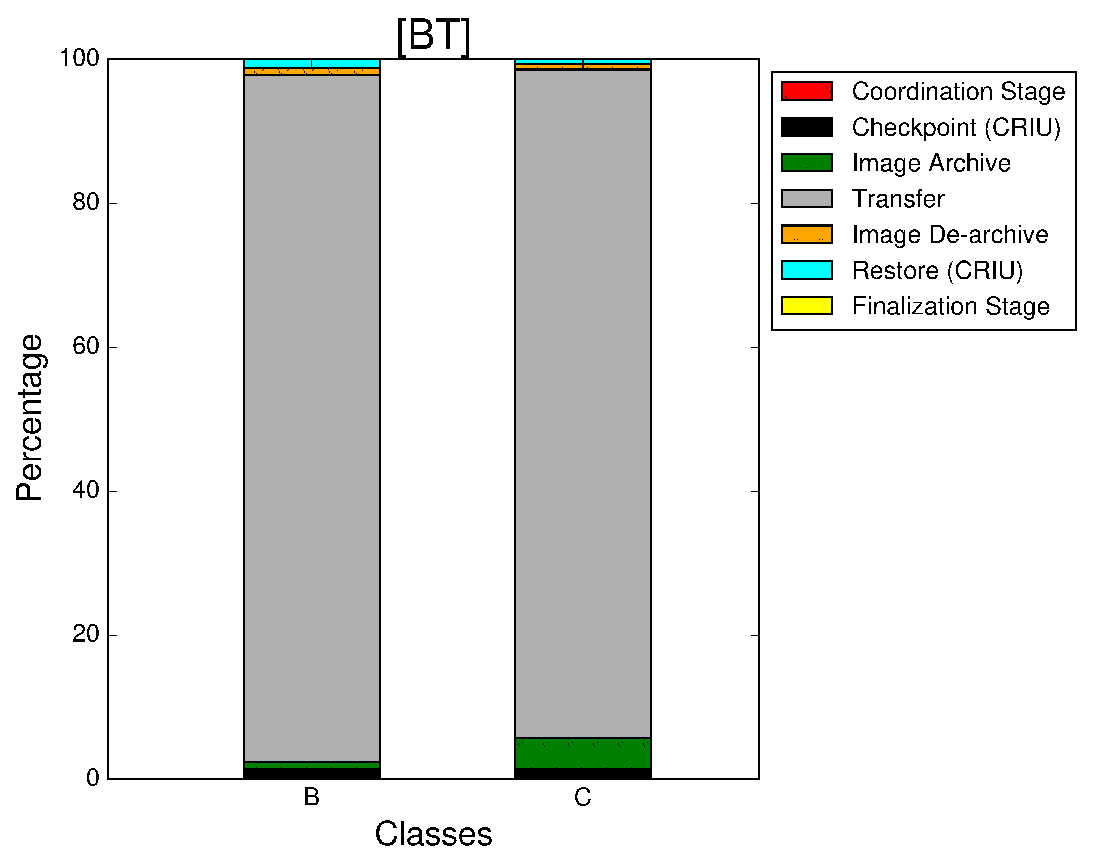
\includegraphics[scale=0.35]{img/migration_comp_bt.eps}
}
\subfloat{%
   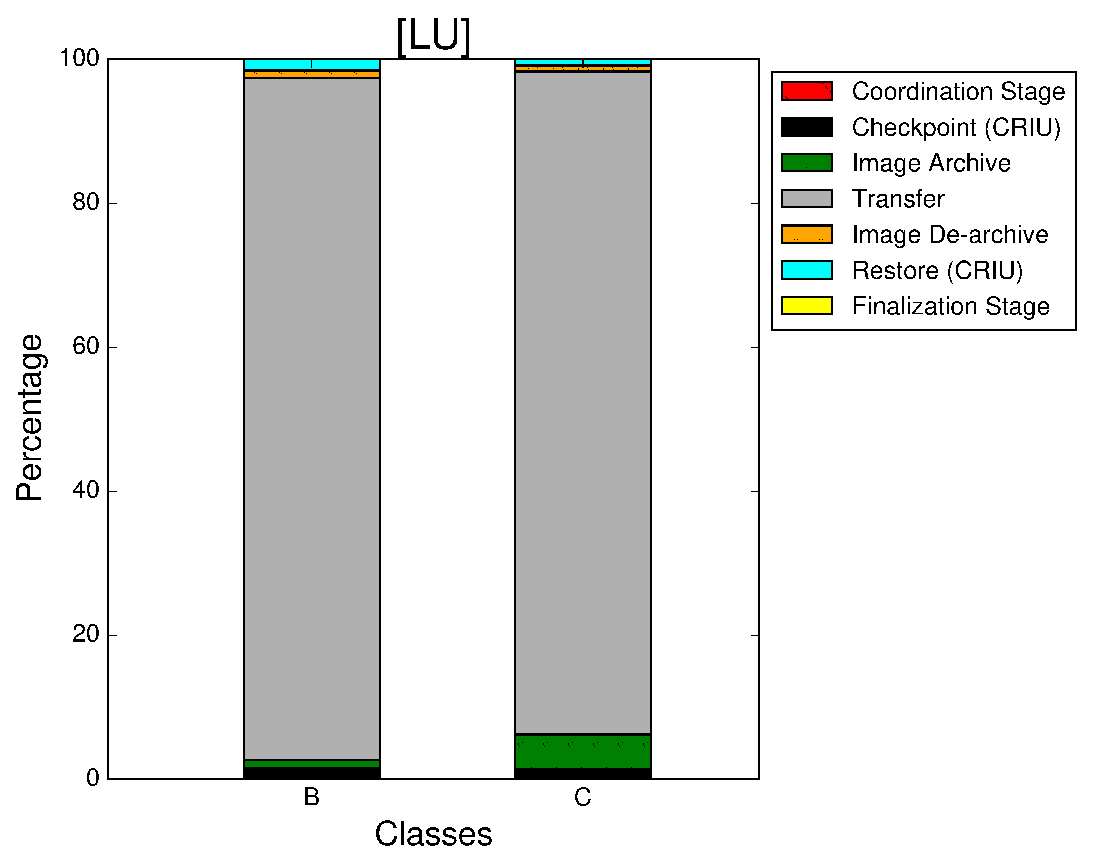
\includegraphics[scale=0.35]{img/migration_comp_lu.eps}
}


\vspace{10pt}

\subfloat{%
   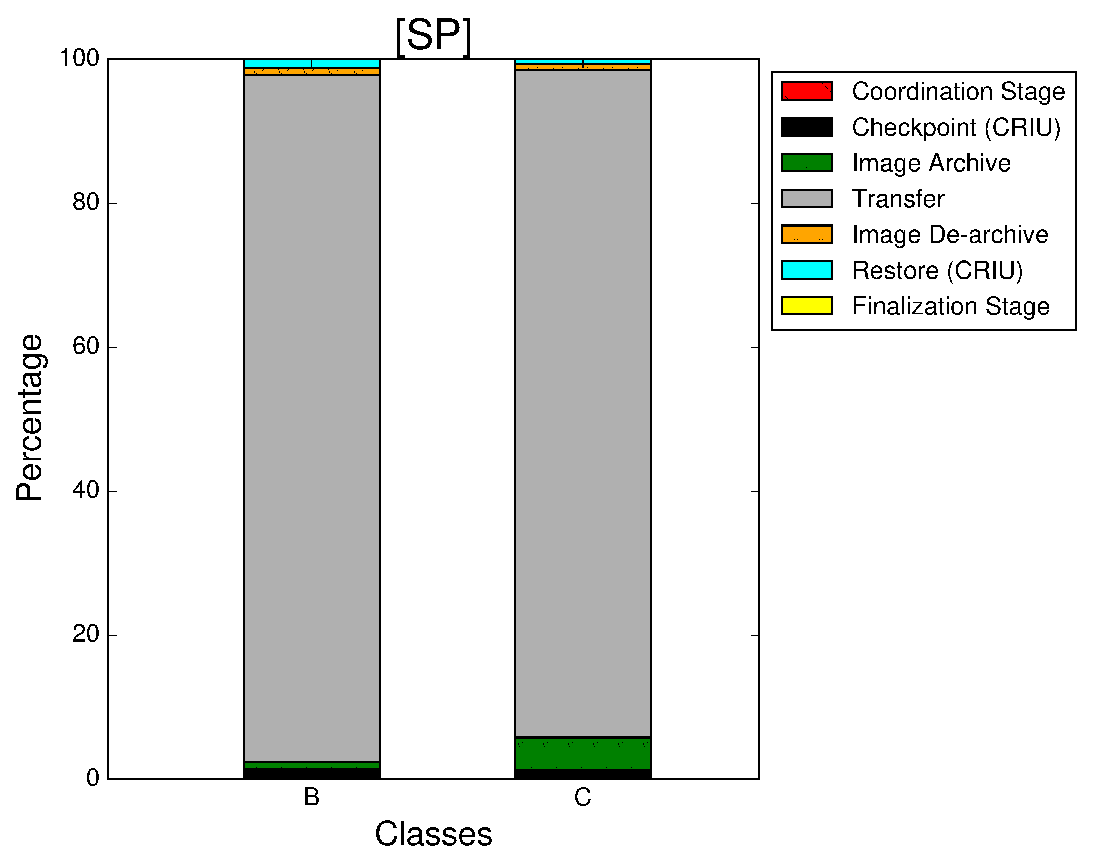
\includegraphics[scale=0.35]{img/migration_comp_sp.eps}
}
\subfloat{%
   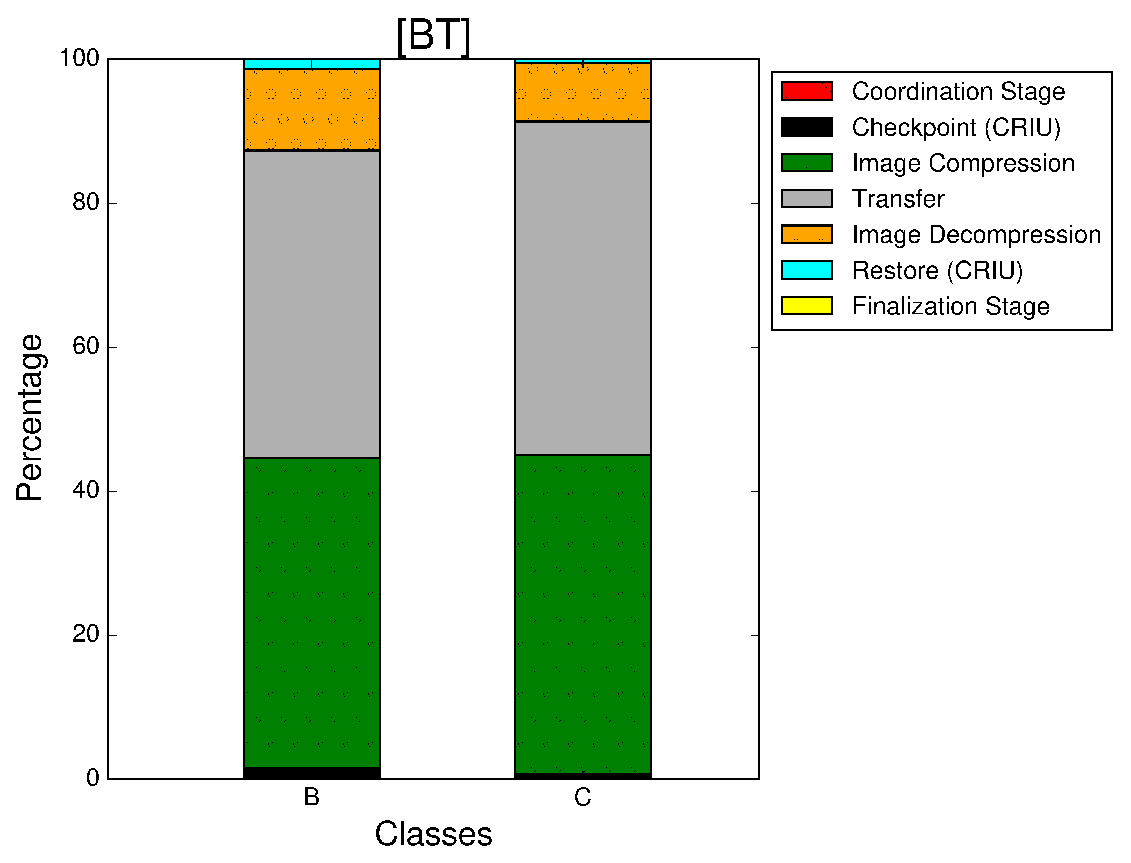
\includegraphics[scale=0.35]{img/migration_comp_bt_gzip.eps}
}

\vspace{10pt}

\subfloat{%
   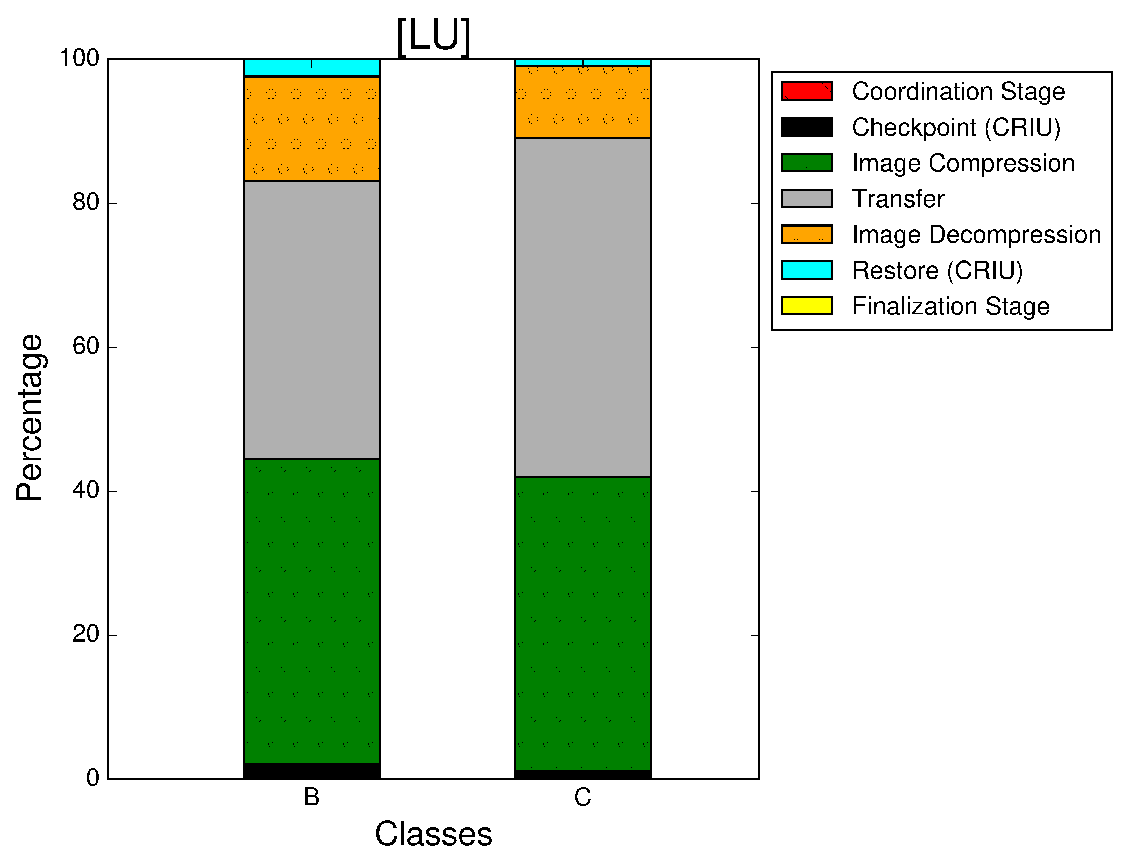
\includegraphics[scale=0.35]{img/migration_comp_lu_gzip.eps}
}
\subfloat{%
   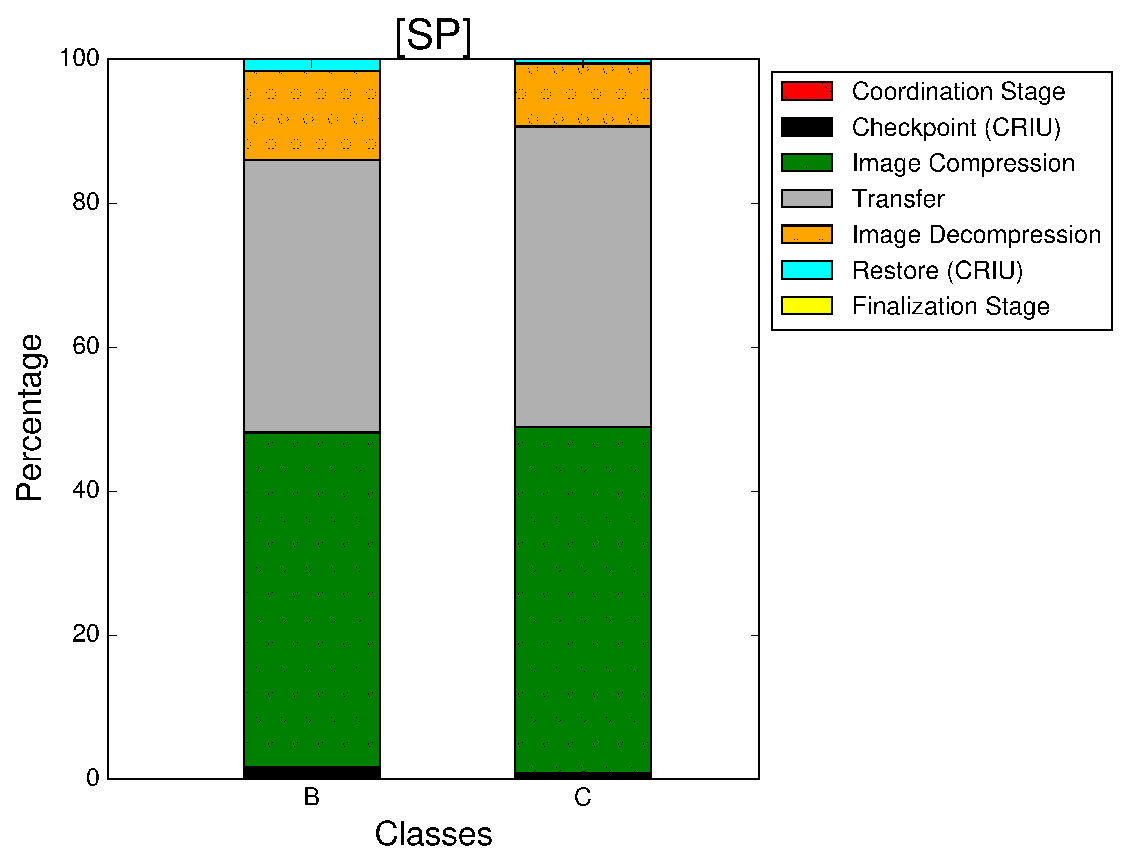
\includegraphics[scale=0.35]{img/migration_comp_sp_gzip.eps}
}
\caption[Process migration time composition]{Process migration time composition with respect to the input problem
size. Top images: migrations without image compression. Bottom figures:
migration  with image compression.}
  \label{fig:migrationstack}%
\end{figure*}

\clearpage

\section{\texttt{mig} : ORTE daemons migration overhead}
\label{sec:migoverhead}
\subsubsection{Hardware setup}
We characterized the migration overhead by
running the benchmarks on two nodes connected via Gigabit Ethernet, both
equipped with two Intel Xeon E5-2640 CPU, 128GB of RAM per CPU (NUMA) and
keeping the Hyper-Threading disabled.

\subsubsection{Methodology}

In the experimental migration scenario, we launched two \emph{ORTE daemon} instances
per node, each one managing 4 out of the 16 application processes. The
resource manager triggered the migration requests after 25 seconds of execution.

To better observe the composition of the migration overhead, we divided the
migration time, isolating seven contributions. We considered the time
required by each of the five migration phases previously described in \ref
{sec:cap4-migphases}, plus two additional contributions:
\begin{enumerate}
\item Time required to encapsulate the CRIU process dump into the archive;
\item Time to extract the dump from the archive after the migration.
\end{enumerate}

With the exception of the \emph{Coordination} and the \emph{Finalization}
phases, the other contributions are expected to be strongly dependent on the
problem size, in particular on the image transfer time.
In this regard, we evaluated the possibility of introducing the compression of
the image generated by the CRIU checkpoint before proceeding with the transfer.
In such a case, a decompression step is obviously required on the destination
node, before resuming the execution of the processes. To this purpose, we
used the GZIP compression algorithm \cite{deutsch1996gzip}.

\subsubsection{Results}

In Figure \ref {fig:cap6-imagesize}, we can see how the compression is effective in
reducing the size of the checkpoint image to transfer. This because of the
shared memory implementation. Open MPI in facts allocates over 100MB of unused
shared memory as ghost files initialized as zeros. The consequence is
that compression is very effective in such cases, resulting in image sizes
scaled down to $22-38\%$ with respect to the original sizes.
In case of bigger datasets instead -- like the \texttt{C} class -- this phenomenon
is less evident, with compressed image sizes resulting the $45-65\%$ of the
original sizes.

\begin{figure}[t]
\centering
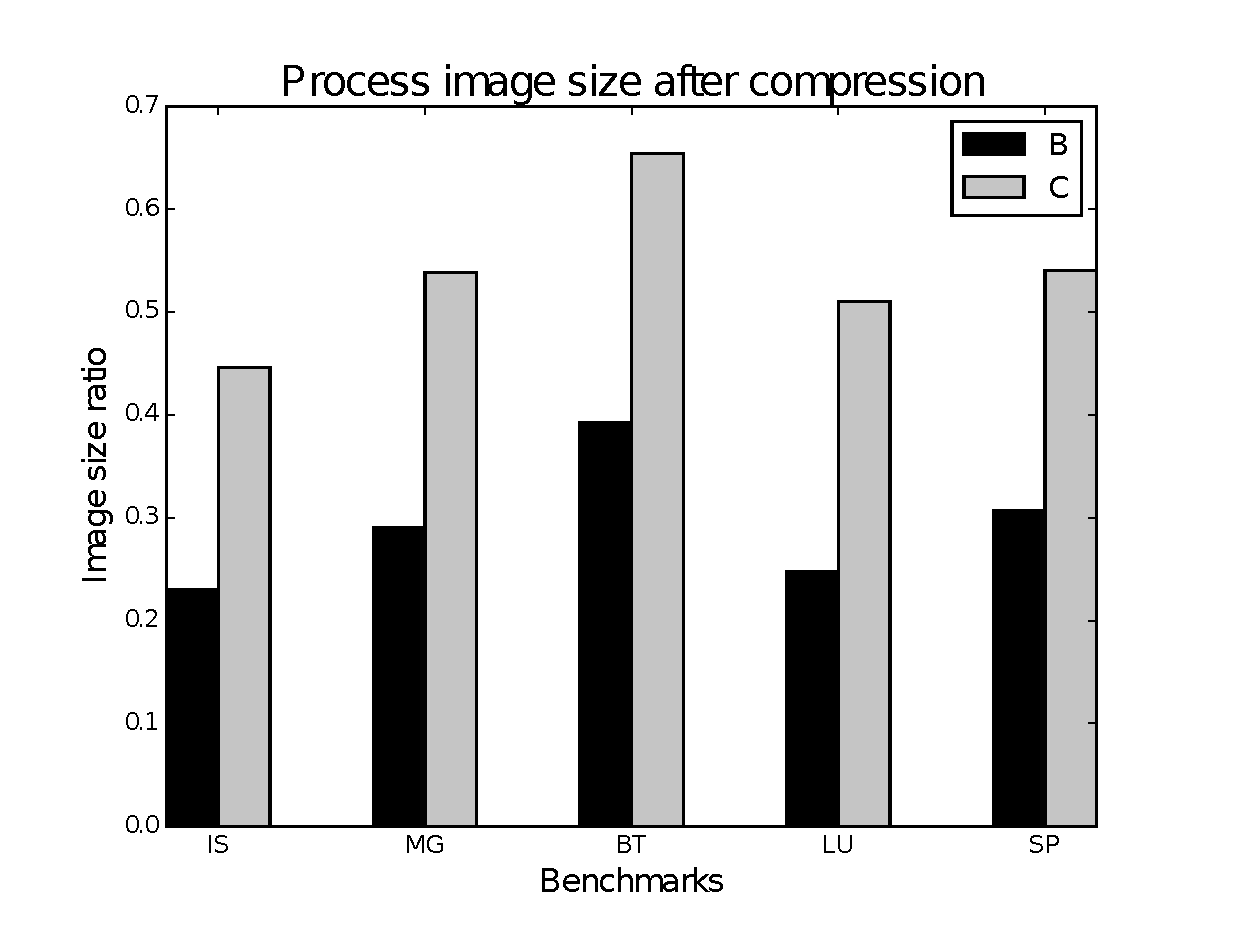
\includegraphics[scale=0.5]{img/image_size_per_data.eps}
\caption[Evaluation of the compression effectiveness]{Process checkpoint image after GZIP compression for each benchmark,
with respect to the input data class}
  \label{fig:cap6-imagesize}%
\end{figure}

The composition of the migration overhead is highlighted in Figure \ref
{fig:migrationstack}. If the compression is not applied (top figures), the time
required to transfer the process image over the network dominates the whole
migration process ($80-90\%$ of the time) independently of the benchmark and
of the class of input data. The contributions due to the synchronization stages
(\emph{Coordination} and \emph{Finalization}) and the time needed for doing
checkpoint/restore with CRIU are instead negligible.

Conversely, when the compression is applied (bottom figures), the transfer time
is reduced, but a new overhead contribution is introduced. The time spent to
perform image compression/decompression is not negligible. We can
observe indeed an overall percentage value comparable to the transfer time
($40-50\%$) for the compression, plus a $10-15\%$ for the decompression.

Figure \ref{fig:cap6-migrationtime} provides an overview of the
measured migration times, comparing the cases with image compression against
cases where no compression is applied. For the \texttt{IS} and \texttt{MG}
benchmarks, where hundreds of MB of data must be moved, the compression
represents a penalty. Conversely, for \texttt{BT}, \texttt{LU} and \texttt{SP},
where data size is a few MB, break-even points can be found.
Generally, we can state that resource manager should be in charge of choosing
whether apply compression or not, taking into account application properties, input
data size, node capabilities and network parameters (e.g., topology, bandwidth,
etc\dots). The \texttt{mig} framework is then driven accordingly.

\subsubsection{Comments}
Please note that these tests were performed on two computational nodes connected
via Gigabit Ethernet. Most recent HPC systems connect nodes using InfiniBand,
which is much faster than Ethernet. It follows that, in the average case, we do
not expect compression to be needed, because transfer time will usually be in
the range of seconds rather than of tens of seconds. In our experimental set-up,
as shown in the results, the time required to interrupt the execution of a set
of processes, to migrate them to another node and to resume their execution is
not negligible and may require tens of seconds.

%%% Migration time
\begin{figure*}[t]
\centering

\subfloat{%
   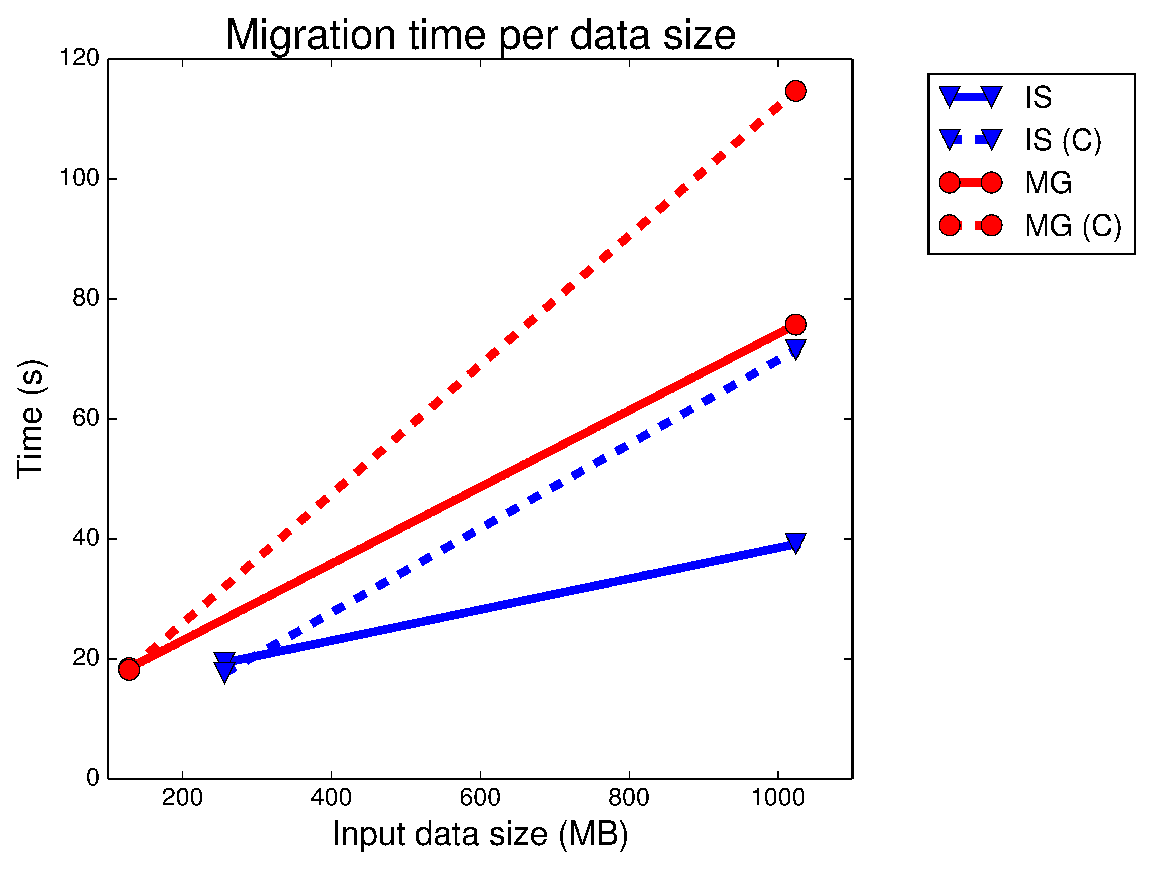
\includegraphics[scale=0.5]{img/migration_time_per_data_im.eps}
}
\hspace{10pt}
\subfloat{%
   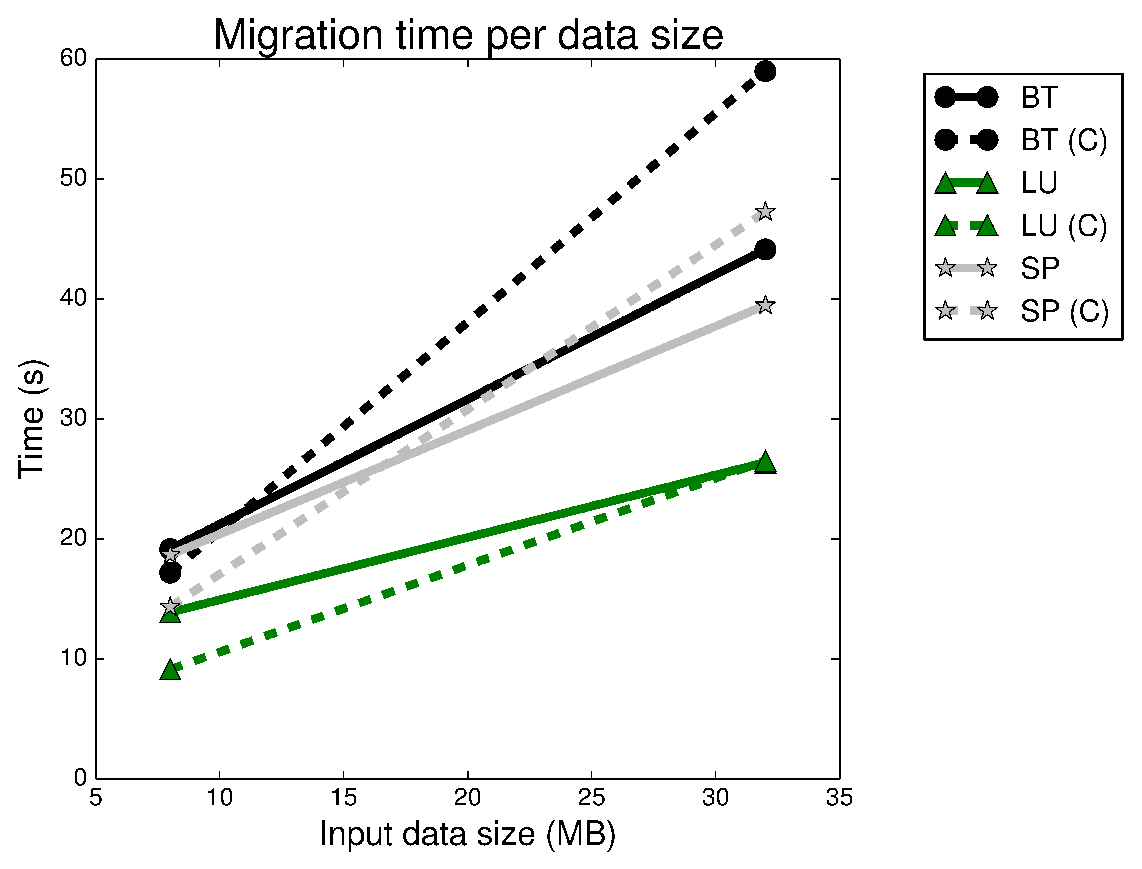
\includegraphics[scale=0.5]{img/migration_time_per_data_bls.eps}
}
\caption[Migration overhead evaluation]{\texttt{IS}, \texttt{MG} and \texttt{BT}, \texttt{SP}, \texttt{LU}
    migration overhead with respect to the input problem size. Migrations using image
    compression (dashed lines (C)) can be compared to migrations without image
    compression.}
  \label{fig:cap6-migrationtime}%
\end{figure*}

\clearpage

\section{DistRib validation}
\label{sec:distribval}

\begin{figure}[t]
    \centerline 
{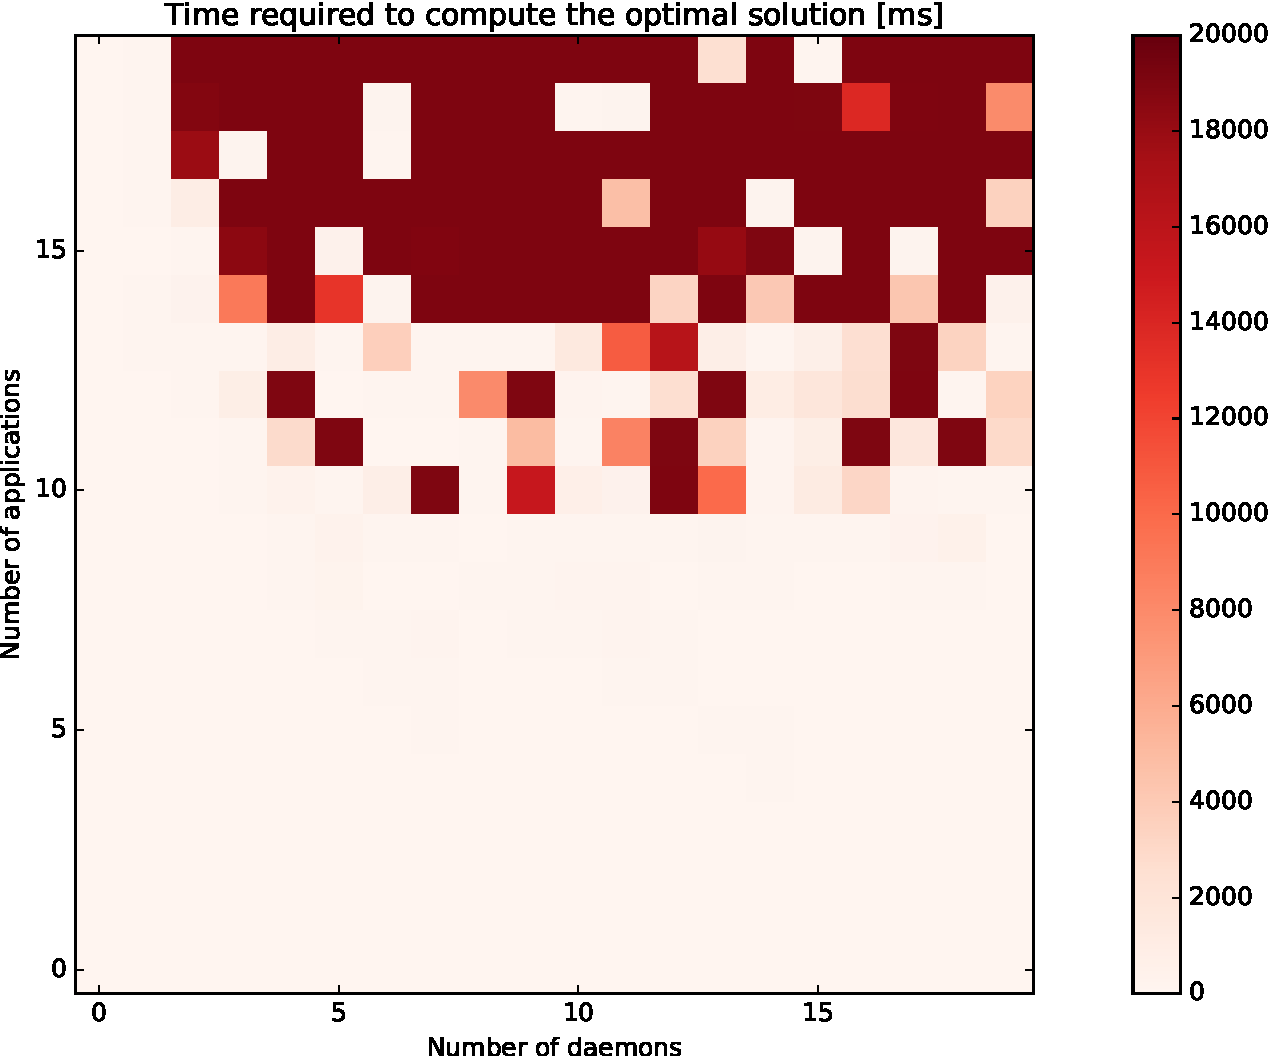
\includegraphics[scale=0.4]{img/ilp-1-cropped.pdf}}
    \caption[DistRib ILP performance (no per-system penalty)]{Performance results of ILP problem with homogeneous systems (no
    per-system penalty).}
    \label{fig:cap5-ilp_nopen}
\end{figure}


\begin{figure}[t]
    \centerline 
{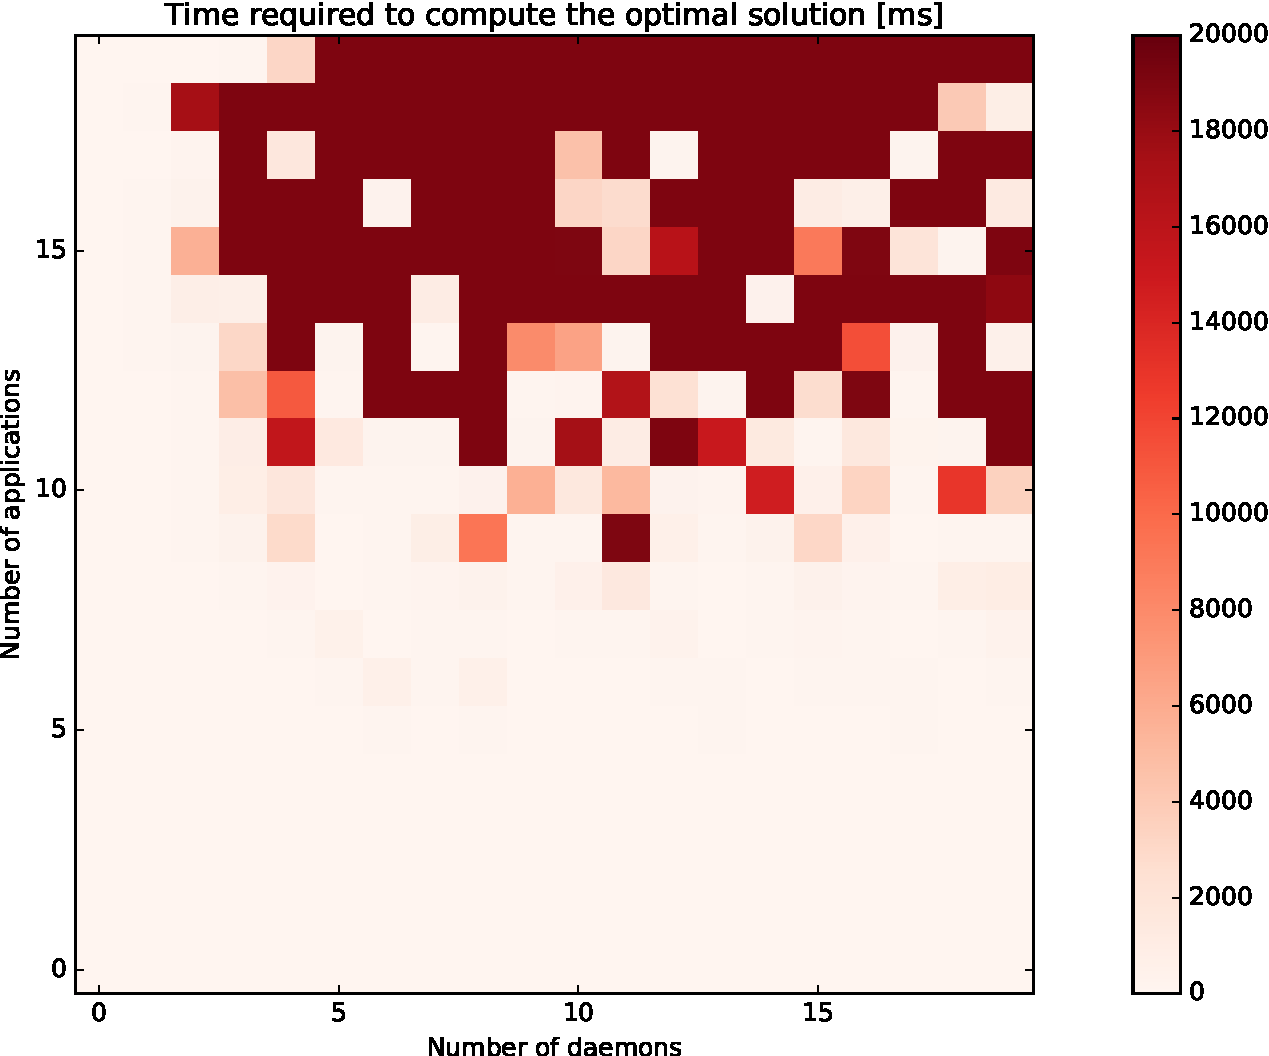
\includegraphics[scale=0.4]{img/ilp-2-cropped.pdf}}
    \caption[DistRib ILP performance (per-system penalty)]{Performance results of ILP problem with heterogeneous systems 
    (per-system penalty presents).}
    \label{fig:cap5-ilp_pen}
\end{figure}

\subsection{The GLPK solver}
In order to solve the ILP problem the
\textbf{GNU Linear Programming Kit (GLPK)}
\cite{makhorin2008glpk} is used. GLPK implements Linear Programming (LP) and
Mixed Integer Programming (MIP) solvers. The latter is a generalized case of 
ILP, since it allows the mix between integer and real variables. Since the
textual formulation presented in Appendix \ref{app:distrib-ilp-formulation}
is adequate
only for the first prototype of the ILP formulation, the actual code uses the 
API provided by GLPK itself, linking the relative shared library.

\subsubsection{The algorithms used}
GLPK implements several algorithms for the resolution. The policy uses the
standard \emph{Simplex algorithm} for solving the LP relaxation and then the
\emph{branch-and-cut} method \cite{mitchell2011branch} to obtain the integer
solutions. The \emph{branch-and-cut} method is a hybrid of classical
\emph{branch-and-bound} and \emph{cutting plane} methods that assure an
optimal solution with a good probability. GLPK allows the production of a 
sensitivity report in order to analyze the goodness of the solution, however
at present this is not used in our software.

\subsection{Performance}

Integer Linear Programming is proved to be \emph{NP-complete}
\cite{papadimitriou1981complexity}, thus no\linebreak polynomial-time
algorithm is known.

We performed the tests timing GLPK solver.
The instances are selected from 1 to 20 systems and from 1 to 20 applications,
for a total of 400 instances. The number of cores per system and the number
of cores per application are uniformly randomized. Each instances are executed
20 times and the resulting execution times have been averaged. A timeout at
20 seconds is placed, after that the execution is killed.

The first batch of tests are executed with \(r_s=0\ \forall s \in S\)
(homogeneous systems) and the results presented in Figure
\ref{fig:cap5-ilp_nopen}. The second batch
of tests are executed with \( r_s \) as a random value from 1 to 10
uniformly distributed. This test implements the case of heterogeneous systems and its results presented in Figure 
\ref{fig:cap5-ilp_pen}.
The two cases do not show any significant difference adding the addend of
per-system penalty to the objective function.

However, GLPK performs well with our ILP programming for number of applications
less than 10, and it seems not very sensitive to the number of systems.
Isolated cases are very fast even with a high number of systems and
applications. For example, \emph{(15 applications, 17 systems)} is very fast
case, but \emph{(14 applications, 17 systems)} and \emph{(16 applications,
17 systems)} are very slow. This behavior may be explained analyzing the
optimization performed by GLPK, that can solve rapidly some special cases.

In a real HPC scenario with thousands of nodes and several applications
a greedy policy or other non optimal algorithm is required. The policy has to
be sufficiently fast in order to do not introduce more overhead.

